\documentclass{beamer}[fullspacing]
\usetheme{Frankfurt}
\usepackage{lmodern}
\usepackage{hyperref}

%\parskip=6pt
%\itemindent=0pt
%\listparindent=0pt

\author{Jianmeng Yu}
\institute{Supervised by: Bob Fisher}
\title{Parallel Massive Dataset Cleaning}
\date{}

\begin{document}

\begin{frame}
\titlepage
\end{frame}


\begin{frame}
\tableofcontents
\end{frame}


\section{Introduction}

\subsection{Motivation}
\begin{frame}
\frametitle{Project Motivation}

\begin{itemize}
\item What is Motivation of the Project?
\begin{itemize}
\item 
1.6 TB dataset, 839 million detections. 
\item
About 60\% are False Positives.
\item
Pugh\cite{Pugh}'s prototype cleaning algorithm.
\item Not applied due to cost (800,000 hours)\cite{Yu}.
\end{itemize}
\item The Goal of this project?
\begin{itemize}
\item
Apply the cleaning algorithm.
\item 
Need a parallel framework to reduce time.
\item 
Need to translate the code.
\end{itemize}
\end{itemize}

\end{frame}



\subsection{Background}

\begin{frame}
\frametitle{Background - Dataset}

\begin{itemize}
\item
Fish4Knowledge (F4K)\cite{F4K} collected 5 years of fish video.
\item
They reduce the recording to 1.6 TB size.
\item
500 GB {\tt .sql} dump, 1.1 TB video and summary csv files.
\end{itemize}

\begin{figure}
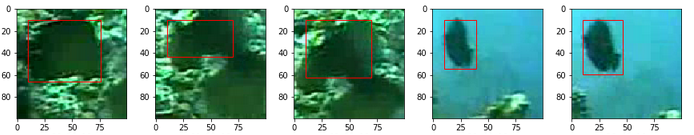
\includegraphics[scale=0.4]{image/sample.png}
\caption{Sample frames of the videos}
\end{figure}

\end{frame}



\begin{frame}
\frametitle{Background - Cleaning Algorithm}

\begin{columns}
\column{0.59\textwidth}
\begin{itemize}
\item
Developed by Matthew Pugh\cite{Pugh}. 
\item
Use Python script to extract info from video/summary.
\item
FEIF to remove some partial-fish before classify.
\item
Feature extraction, transformation for SVM.
\item 
Transformation and normalize image for CNN.
\item
Use Top-N algorithm to obtain decision vector.
\end{itemize}

\column{0.41\textwidth}
\begin{figure}
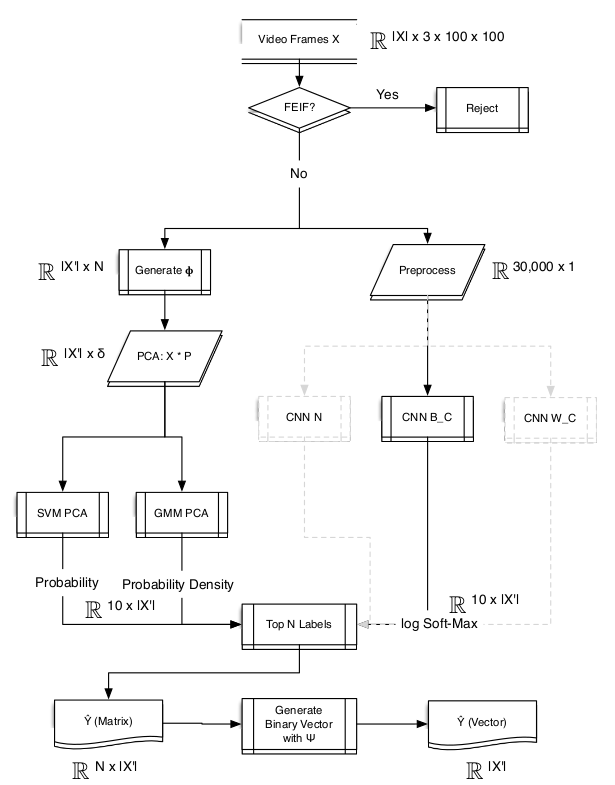
\includegraphics[scale=0.2]{image/pipe.png}
\caption{Pipeline Classifier}
\end{figure}
\end{columns}

\end{frame}



\subsection{Main Problems}

\begin{frame}
\frametitle{Project Problems}

The project has encountered several problems on the algorithm:
\begin{itemize}
\item
The pipeline is only tested without parallelization.
\item
Dump file top large for school PostgreSQL service.
\item
Ambiguous classification schema.
\item
Training data wasn't representative.
\item
Extreme runtime cost - even for 200 DICE machines.
\item
Translation needed, for more portability.
\item
CNN trained is broken, over-fits on badly transformed dataset. 
\item
Prototype stage - The best Top-N strategy is not found.
\end{itemize}

\end{frame}



\section{Details of Problems and Solution}
\subsection{Parallel Distribution}

\begin{frame}
\frametitle{Details - Parallel Distribution}

The first challenge is the distribution of the task.
\begin{itemize}
\item
220 student lab DICE machines.
\item
800 cores reduces runtime significantly.
\item
A Python script is used to ``scan'' for idle machines.
\item
University provides a shared file system (AFS).
\item
MPI is used for the communication between process.
\end{itemize}

\begin{figure}
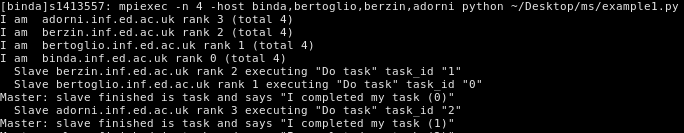
\includegraphics[scale=0.4]{image/mpi.png}
\caption{Framework Example Run}
\end{figure}

\end{frame}



\subsection{Data Extraction from SQL dump file}

\begin{frame}
\frametitle{Details - Standard I/O Stream Extraction}

Another problem of the project is the lack of a SQL server.
\begin{itemize}
\item
500 GB {\tt .sql} dump file too large for PostgreSQL service.
\item
Independent records, SQL query may not be best choice.
\item
Alternatively, parse relevant information to csv file.
\item
Saves time and cost for maintaining a server.
\item
Reduces dump file to 2/3 size, also makes loading faster.
\end{itemize}

\end{frame}



\subsection{Frame Edge Indicator Function}

\begin{frame}
\frametitle{Details - Frame Edge Indicator Function}

FEIF removes all of fish touching frame edge.

\begin{columns}
\column{0.5\textwidth}
\begin{itemize}
\item
Reduces dataset by 10\%.
\item
Fast, but reject good fish sometimes.
\end{itemize}

Another similar method is used to reject planktons.

\begin{itemize}
\item
Reject all the videos recorded at night.
\item
These videos have over 99\% of False Positive.
\item
Reduces dataset by 8\%.
\end{itemize}

\column{0.41\textwidth}
\begin{figure}
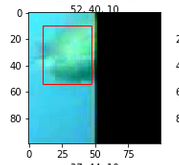
\includegraphics[scale=0.5]{image/FEIF.png}
\caption{Sample Frame Touching Edge}
\end{figure}
\end{columns}

\end{frame}



\subsection{Ground Truthing Dataset}

\begin{frame}
\frametitle{Details - Ground Truth}

\begin{itemize}
\item
Pugh created a 10-class classification schema.
\item
He marked 60,000 detections for training.
\item
Class 6 and 8 are acceptable fishes.
\end{itemize}

\begin{figure}
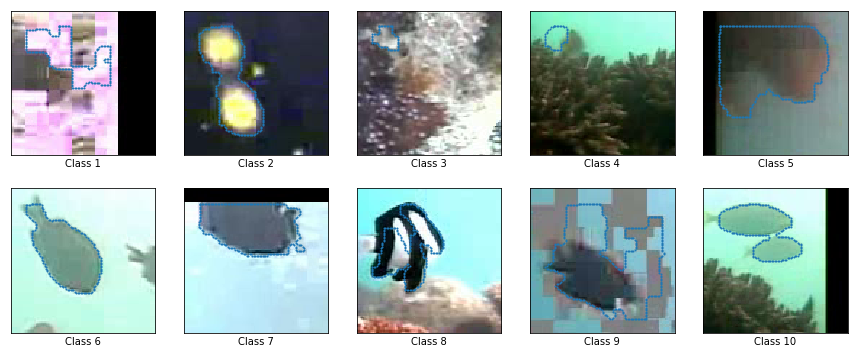
\includegraphics[scale=0.2]{image/class_sample.png}
\caption{Sample fish from each class}
\end{figure}

\vspace{-15pt}
\begin{itemize}
\item
This project marked  another 20,000 detections for validation.
\end{itemize}

\end{frame}



\subsection{Code Translation}

\begin{frame}
\frametitle{Details - Translating MATLAB code into Python}

\begin{columns}
\column{0.59\textwidth}
\begin{itemize}
\item
Most of the pipeline parts are translated into Python.
\item
Except Feature Extraction in MATLAB and CNN in Lua.
\item
After benchmarking, a full translation does not seem optimal.
\item 
PyMatlab and Lutorpy are used instead.
\end{itemize}

\column{0.41\textwidth}
\begin{figure}
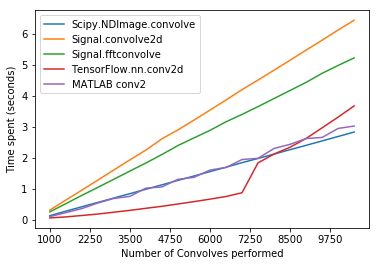
\includegraphics[scale=0.3]{image/benchmark.png}
\caption{Performance of different convolution algorithms}
\end{figure}
\end{columns}

\end{frame}



\subsection{Classifiers}

\begin{frame}
\frametitle{Details - Classifiers}

\begin{itemize}
\item
The SVM performed the as expected.
\item
CNNs trained does not work as intended.
\item
This is caused by color space issues in OpenCV. 
\item
Retraining the CNN too costly and not used.
\end{itemize}

\begin{columns}
\setlength{\abovecaptionskip}{-2pt}
\column{0.5\textwidth}
\begin{figure}
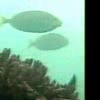
\includegraphics[scale=0.6]{image/outfile.jpg}
\caption{Normal Image in RGB space}
\end{figure}

\column{0.6\textwidth}
\begin{figure}
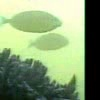
\includegraphics[scale=0.6]{image/outfile2.jpg}
\caption{OpenCV output, in BGR space}
\end{figure}
\end{columns}

\end{frame}



\subsection{Voting Strategy}

\begin{frame}
\frametitle{Details - Voting Strategy}

\begin{columns}
\column{0.6\textwidth}
\begin{itemize}
\item
Uses voting instead of the original Top-N decision.
\item
Use ROC curve to pick strategy.
\item
For keeping most True Positive, use SVM only is the best strategy.
\end{itemize}

\column{0.4\textwidth}
\begin{figure}
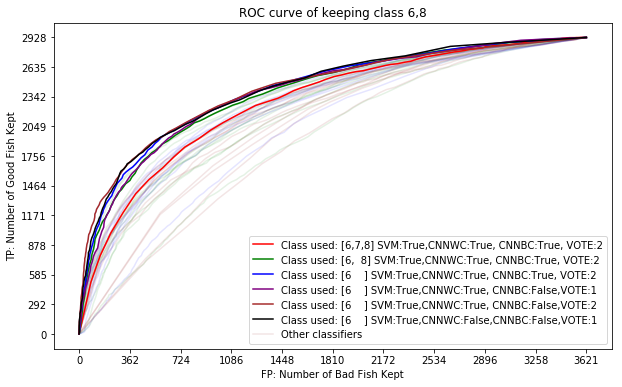
\includegraphics[scale=0.2]{image/roccurve.png}
\end{figure}
\end{columns}
\end{frame}



\section{Results}
\subsection{Project Result}
\begin{frame}
\frametitle{Result - Outcome}

Project Result:
\begin{itemize}
\item
28\% of the 1.6 TB dataset is removed.
\item
40\% of the False Positive rejected.
\item
Finished the task in 11 days of computational time.
\end{itemize}

It does not achieve Pugh's predicted 90\% FP removal.
This is caused by:
\begin{itemize}
\item
CNN over-fit, accuracy drops 20\% on validation set.
\item
Poor coverage on training-set.
\item
Over-estimation due to Pugh's 2-Fold Training/Testing split.
\end{itemize}
\end{frame}



\begin{frame}
\frametitle{Result - Samples}

\begin{itemize}
\item
The SVM appears to learn the shape of detections well.
\item
High probability detections are usually good fish.
\item
FP are mixed with TP with erratic contour.
\end{itemize}
\begin{figure}
\setlength{\abovecaptionskip}{-2pt}
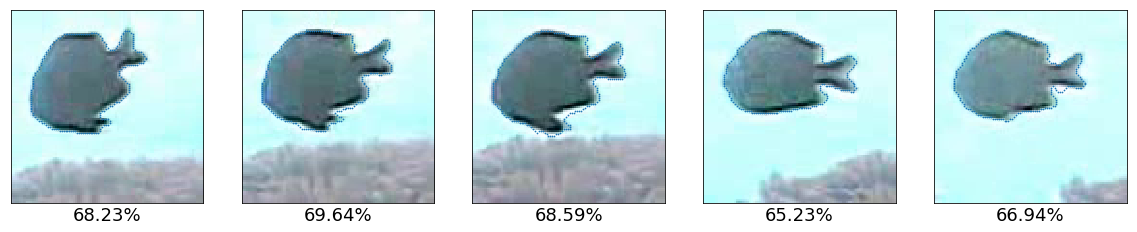
\includegraphics[scale=0.25]{image/HP.png}
\caption{Positives with High Probability}
\end{figure}
\vspace{-10pt}
\begin{figure}
\setlength{\abovecaptionskip}{-2pt}
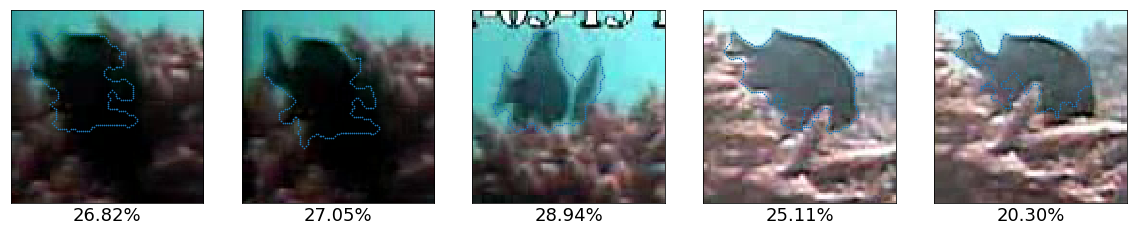
\includegraphics[scale=0.25]{image/LP.png}
\caption{Positives with Low Probability}
\end{figure}

\end{frame}




\begin{frame}
\frametitle{Result - Achievements}

\begin{itemize}
\item
Finishes the 800,000 hour task.
\item
Took about 10 days of computational day.
\item
Estimated 90\% reduction on single-core time cost.
\item
Potentially reduces dataset by 500 GB.
\item 
Removes 40\% of FP at lost of 10\% TP.
\item
Most kept FP have low SVM score.
\item
Most reject TP have very erratic boundary.
\end{itemize}


\end{frame}



\subsection{Future Work}
\begin{frame}
\frametitle{Future Works}
\begin{itemize}
\item
More Ground Truth dataset.
\item
Fix the True Negatives caused by FEIF.
\item
Re-train the CNN used with correct data.
\end{itemize}
\end{frame}


\begin{frame}
\begin{Huge}
\begin{center}
Questions?
\end{center}
\end{Huge}
\end{frame}




\section*{Bibliography}
\setbeamertemplate{bibliography item}{\insertbiblabel}
\begin{frame}
\frametitle{Bibliography}
\begin{thebibliography}{3} % Beamer does not support BibTeX so references must be inserted manually as below
\bibitem{Pugh}
Matthew Pugh.
\newblock Removing false detections from a large fish image data-set.
\newblock Msc dissertation, The University of Edinburgh, 2015.

\bibitem{Yu}
Qiqi Yu.
\newblock Adding temporal constraints to a large data cleaning problem.
\newblock Msc dissertation, The University of Edinburgh, 2016.

\bibitem{F4K}
Robert B Fisher{,} Yun-Heh Chen-Burger{,} Daniela Giordano{,} Lynda Hardman{,}
  Fang-Pang Lin.
\newblock {\em Fish4Knowledge: collecting and analyzing massive coral reef fish
  video data}.
\newblock Springer, 2016.

\end{thebibliography}
\end{frame}

\end{document}